\documentclass[12pt,oneside]{book}
\usepackage{times,mathptmx}
\usepackage[pdftex]{graphicx}
\usepackage{calc}
\usepackage{tabularx,ragged2e,booktabs,caption,subcaption}
\usepackage{array}
\newcolumntype{L}[1]{>{\raggedright\let\newline\\\arraybackslash\hspace{0pt}}m{#1}}
\newcolumntype{C}[1]{>{\centering\let\newline\\\arraybackslash\hspace{0pt}}m{#1}}
\newcolumntype{R}[1]{>{\raggedleft\let\newline\\\arraybackslash\hspace{0pt}}m{#1}}
\usepackage{multirow}
\usepackage{multicol}
\usepackage{tocloft}
\usepackage{xcolor}
\usepackage{color,soul}
\usepackage{amsmath}
\definecolor{linknavy}{rgb}{0,0,0.50196}
\definecolor{linkred}{rgb}{1,0,0}
\definecolor{linkblue}{rgb}{0,0,1}
\definecolor{darkorange}{rgb}{0.81,0.52,0}
\definecolor{fc_orange}{rgb}{0.94,0.59,0.14}
\definecolor{brown}{rgb}{0.56,0.36,0}
\definecolor{fc_blue}{rgb}{0.27,.36,0.48}
\usepackage{float}
\usepackage{graphpap}
\usepackage{rotating}
\usepackage{graphicx}
\usepackage{geometry}
\usepackage{relsize}
\usepackage{ltablex}
\usepackage{longtable}
\usepackage{lscape}
\usepackage{amssymb}
\usepackage{makeidx} % Create index at end of document
\usepackage[nottoc,notlof,notlot]{tocbibind} % Put the bibliography and index in the ToC
\usepackage{lastpage} % Automatic last page number reference.
\usepackage[T1]{fontenc}
\usepackage{enumerate}
\usepackage{upquote}
\usepackage{moreverb}
\usepackage{xfrac}
\usepackage{cite}
\usepackage{tikz}
% \usepackage{subfig}
% \usepackage{caption}
\usepackage[toc,page]{appendix}
\usepackage{notoccite}
\usepackage{placeins}

\usepackage{titlesec}
\titleformat{\chapter}[hang] 
{\color{fc_blue}\normalfont\huge\bfseries}{\chaptertitlename\ \thechapter}{1em}{}[\titlerule]
\titlespacing*{\chapter}{0pt}{-30pt}{20pt}

\titleformat*{\section}{\normalfont\Large\bfseries\color{fc_blue}}
\titleformat*{\subsection}{\normalfont\large\bfseries\color{fc_blue}}

\newcommand{\nopart}{\expandafter\def\csname Parent-1\endcsname{}} % To fix table of contents in pdf.

\usepackage{siunitx}
\sisetup{
    detect-all = true,
    input-decimal-markers = {.},
    input-ignore = {,},
    inter-unit-product = \ensuremath{{}\cdot{}},
    multi-part-units = repeat,
    number-unit-product = \text{~},
    per-mode = fraction,
    separate-uncertainty = true,
}

\usepackage{listings}
\usepackage{textcomp}
\definecolor{lbcolor}{rgb}{0.96,0.96,0.96}

\usepackage[pdftex,
        colorlinks=true,
        urlcolor=fc_orange,     % \href{...}{...} external (URL)
        citecolor=fc_orange,     % citation number colors
        linkcolor=fc_orange,    % \ref{...} and \pageref{...}
        pdfproducer={pdflatex},
        pdfpagemode=UseNone,
        bookmarksopen=true,
        plainpages=false,
        verbose]{hyperref}

\renewcommand{\cftchapfont}{\hypersetup{linkcolor=fc_blue}}
\renewcommand{\cftsecfont}{\hypersetup{linkcolor=black}}
\renewcommand{\cftsubsecfont}{\hypersetup{linkcolor=black}}
\renewcommand{\cftsubsubsecfont}{\hypersetup{linkcolor=black}}


\setlength{\textwidth}{6.5in}
\setlength{\textheight}{9.0in}
\setlength{\topmargin}{0.in}
\setlength{\headheight}{0.pt}
\setlength{\headsep}{0.in}
\setlength{\parindent}{0.0in}
\setlength{\itemindent}{0.25in}
\setlength{\oddsidemargin}{0.0in}
\setlength{\evensidemargin}{0.0in}
% \setlength{\leftmargini}{\parindent} % Controls the indenting of the "bullets" in a list
\setlength{\cftsecnumwidth}{0.45in}
\setlength{\cftsubsecnumwidth}{0.5in}
\setlength{\cftfignumwidth}{0.45in}
\setlength{\cfttabnumwidth}{0.45in}
\setlength{\parskip}{1em}

% \newcolumntype{L}{>{\centering\arraybackslash}m{4cm}}

\floatstyle{boxed}
\newfloat{notebox}{H}{lon}
\newfloat{warning}{H}{low}

\newenvironment{conditions}
  {\par\vspace{\abovedisplayskip}\noindent\begin{tabular}{>{$}l<{$} @{${}={}$} l}}
  {\end{tabular}\par\vspace{\belowdisplayskip}}


% Rename chapter headings
\renewcommand{\chaptername}{}
\renewcommand{\bibname}{References}

\usepackage{fancyhdr}
\pagestyle{fancy}
\lhead{}
\rhead{}
\chead{}
\renewcommand{\headrulewidth}{0pt}

\usepackage{draftwatermark}
\SetWatermarkText{DRAFT}
\SetWatermarkScale{1}

\begin{document}
\pagenumbering{gobble}

\bibliographystyle{unsrt}
%\pagestyle{empty}

\frontmatter

\begin{minipage}[t][9in][s]{6.25in}
\pagenumbering{gobble}


\headerB{
FireCARES \\
User and Implementation Guide \\
}

\headerC{
\flushleft{Version 1.5}
\flushleft{\today \\}
}

\vfill

\flushright{
\includegraphics[width=2in]{Figures/firecares-header-logo}}

\titlesigs

\end{minipage}

\frontmatter

\pagestyle{plain}
\pagenumbering{roman}

\newpage

\cleardoublepage
\phantomsection
\addcontentsline{toc}{chapter}{Contents}
\tableofcontents

\cleardoublepage
\phantomsection
\addcontentsline{toc}{chapter}{List of Figures}
\listoffigures

\cleardoublepage
\phantomsection
\addcontentsline{toc}{chapter}{List of Tables}
\listoftables

\chapter{List of Acronyms}

\begin{tabbing}
\hspace{1.5in} \= \\

IAFF \> International Assocation of Fire Fighters \\
UL FSRI \> UL Firefighter Safety Research Institute \\
NIST \> National Institute of Standards and Technology  \\
\end{tabbing}

\newpage
\mainmatter

\chapter{Introduction to FireCARES}
A fire department's relationship with data and performance should be seen as a continuum. Statements regarding department's need to have ``good data'' and ``good performance'' are numerous. However, these statements are not the same thing. The beginning of the quality performance continuum is for a department to have ``good data''. Good data is defined as data that are based on factual incidents, reported accurately, and can be accessed and manipulated easily. It can take a department a long time to work on their data but it's important to recognize their ability to quantify impact before instituting change. Without good data there is no assurance that improvement efforts actually work.

Once a department has improved their data quality, they can begin working on having ``good performance.'' Good performance is the end of the quality improvement continuum. For example, improving fire station layouts to reduce turnout time, working with the communications center to streamline call processing, conducting targeted staff training, investing in community risk reduction efforts, and deploying additional/alternate resources within a jurisdiction are all ways to improve performance. 
A knee jerk reaction to observing a given performance metric for a department may be to say that ``the metric is wrong.'' However, in determining the root cause, it is important to distinguish whether the data used in the calculations are wrong or the performance itself is poor.  

FireCARES (firecares.org) is designed to analyze how fire department resources are deployed to match community risks. Local government decision makers often alter fire department resources faster than fire service leaders can evaluate the potential impact. These decisions can leave a community without sufficient resources to respond to emergency calls safely, efficiently, and effectively. These decisions can have even greater impact on vulnerable populations including the elderly, young children, and people with disabilities. FireCARES - Community Assessment, Response Evaluation System - is an analytical system designed to evaluate community risk and fire department operational performance using national data layers in a geographic-based system. The FireCARES project provides fire departments the ability to add a technical basis to what has historically been an anecdotal discussion regarding community hazards and risks as well as the impact of changes to fire department resource levels.

The goal of the project is to aggregate national and local data to provide answers that both public and fire service leaders have not previously had. To accomplish this task, FireCARES provides three scores for each community dependent on the available data: the Community Risk Score, the Fire Department Performance Score, and the Safe Grade.

\section{Community Risk}

The community risk score was developed as a function of the socio-demographic and geographic characteristics of the locations (census tracts) of reported structure fires over a seven year period (2008-2014) according to available NFIRS data. The socio-demographic attributes include:

\begin{itemize}
\item Population characteristics (e.g., size category of the department, population, number of males, age group counts, race counts)
\item Housing characteristics (e.g., total housing units, total vacancies, size of home, number of renters, age of units)
\item Household characteristics (e.g., median household income, social vulnerability index)
\item Geographic region
\end{itemize}

\section{Fire Department Performance Score}

The goal of the fire department performance score is to assess how well a fire department performs compared to the ``standardized'' version of itself. One component of this metric is the structure fire spread category from the National Fire Incident Reporting System (NFIRS). This category provides information which quantifies the fire spread in a structure from confined to object of origin through spread beyond structure of origin. There are five categories defined in NFIRS, but for this analysis the data are collapsed into three categories: room of origin (lumping object and room together), floor of origin (lumping floor and structure together), and beyond structure of origin. The resulting distribution (count of fires in each of the three bins) of fire spread is the basis for comparison for developing the performance score.

The second component of this score is the model that defines how the fire department would perform if it were acting as a standard, idealized version of itself. The concept is that there exists a theoretical version of every fire department where all responses meet or exceed the national standards governing department performance. Essentially, a fire department responding to a fire must complete a series of tasks before they can put water on the fire. For purposes of this model these tasks are broken up as follows:

\begin{itemize}
\item Time to alarm - Time required before the fire is noticed, and some form of action is taken [NIST TN 1661, NIST TN 1797]
\item Time to dispatch - Time required for dispatch operator to obtain enough information regarding the fire and location to issue a dispatch [NFPA 1710]
\item Time to turnout - Time required for firefighter turnout [NFPA 1710]
\item Time to arrival - Transit time required for engine between station and fire location [NFPA 1710, GIS]
\item Time to ascend - Transit time required for firefighters to ascend to the staging floor for fires in buildings. Data for ascent was gathered from timed 27-story climb experiments with 35 firefighters of varying age, height, weight, and gender. Note this parameter is only enacted when staging would occur above ground level.
\item Time to suppress - Time required for firefighters on-scene to put water onto fire (includes size-up, hose connection, etc.) [NIST TN 1661, NIST TN 1797]
\end{itemize}

When water is put onto a fire, the idealized fire is assumed to have reached the peak size. The growth time for the fire is equivalent to the sum of the tasks the fire department must perform to suppress the fire. This time to suppression is coupled to a simple exponential area damage growth model which is consistent with fire statistics literature. A distribution of fire spread is generated using the same three NFIRS bins discussed above, based on the modeled area of fire damage at the suppression time. Distributions of the room and building sizes are estimated from the American Housing Survey's (AHS) national survey of residential homes. Where available, it is possible to use the AHS metropolitan statistical areas to refine room and building distributions for larger metropolitan areas.

The concept is that there exists an average time correction for all fire department structure fire responses routed through the idealized fire department model that ``corrects'' the fire damage outcomes expected from national standards to the particular outcomes observed by a given fire department. This average correction time is known as the fire department performance score.

\section{Safe Grade}

A community's set of safe grades represent an assessment of the number of fires, of fire spread, and of civilian and firefighter injury or death based on how well the Fire Department resources (performance score) match the level of risks within the community (risk score). There are 3 safe grade comparison categories:

\begin{itemize}
\item Performance based on number of fires
\item Performance based on fire spread
\item Performance based on injury and death
\end{itemize}

There are three Safe Grades in total. The Safe Grades compare the local department against similar departments a based on the risk group (low, medium, high) the community falls within for the respective category (see above).


\chapter{Using the Website Features}

\section{Fire Department Landing Page}

\begin{figure}[ht!]
\centering
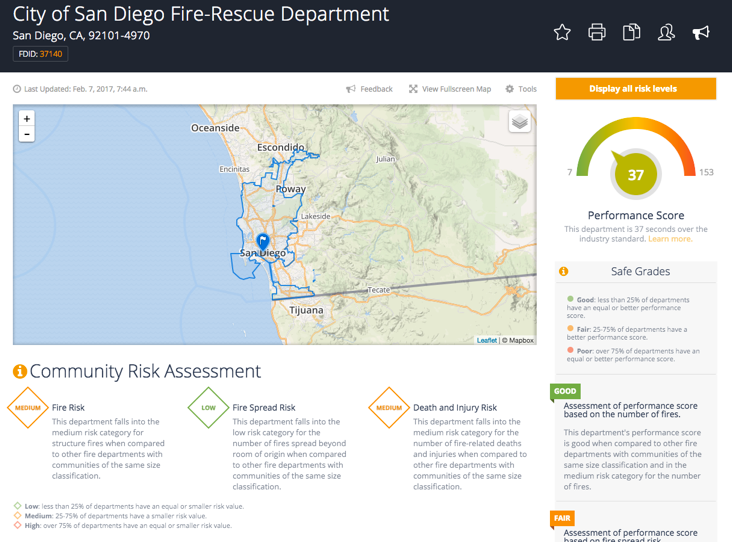
\includegraphics[width=.9\columnwidth]{Figures/department_page}
\caption{FireCARES department landing page}
\label{fig:department_page}
\end{figure}

When viewing your department's page, the first item to check is to ensure that your department's juridictional boundary (the blue outline in Figure~\ref{fig:department_page}) is present and correct. If you notice differences or if boundaries have changed, please send an email to: \href{mailto:boundaries@firecares.org}{Jurisdictional Boundaries}. Be sure to include your Fire Department Name and FDID as it is specified on \href{https://www.FireCARES.org}{FireCARES.org}.


\subsection{Department Details}

\subsection{Annual Structure Fires}

\begin{figure}[ht!]
\centering
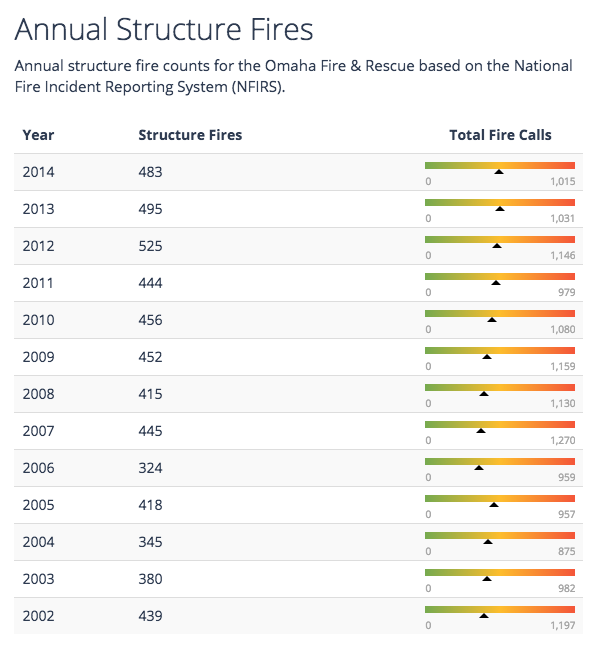
\includegraphics[width=.65\columnwidth]{Figures/structure_fires}
\caption{Annual counts of structure fires (completed structure fire module in NFIRS and total fire calls).}
\label{fig:structure_fires}
\end{figure}

\section{Station Detail Page}

\begin{figure}[ht!]
\centering
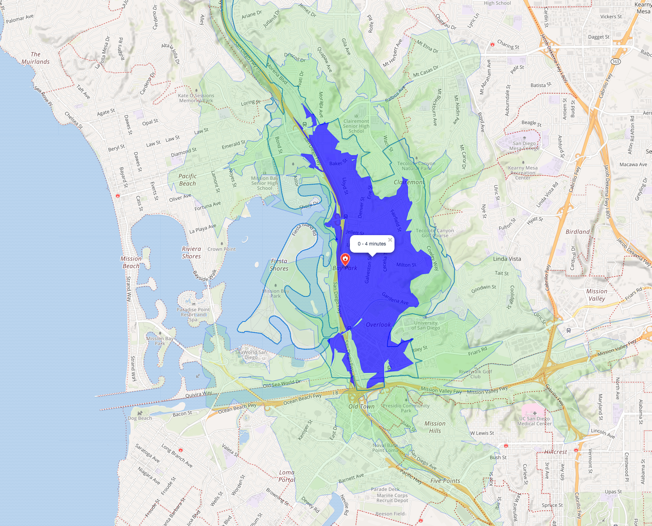
\includegraphics[width=.9\columnwidth]{Figures/response_area}
\caption{GIS based response polygons for 0-4 minute travel times, 4-6 minute travel times, and 6-8 minute travel times.}
\label{fig:response_area}
\end{figure}

\section{Interactive Fires Heat Map}

\begin{figure}[ht!]
\centering
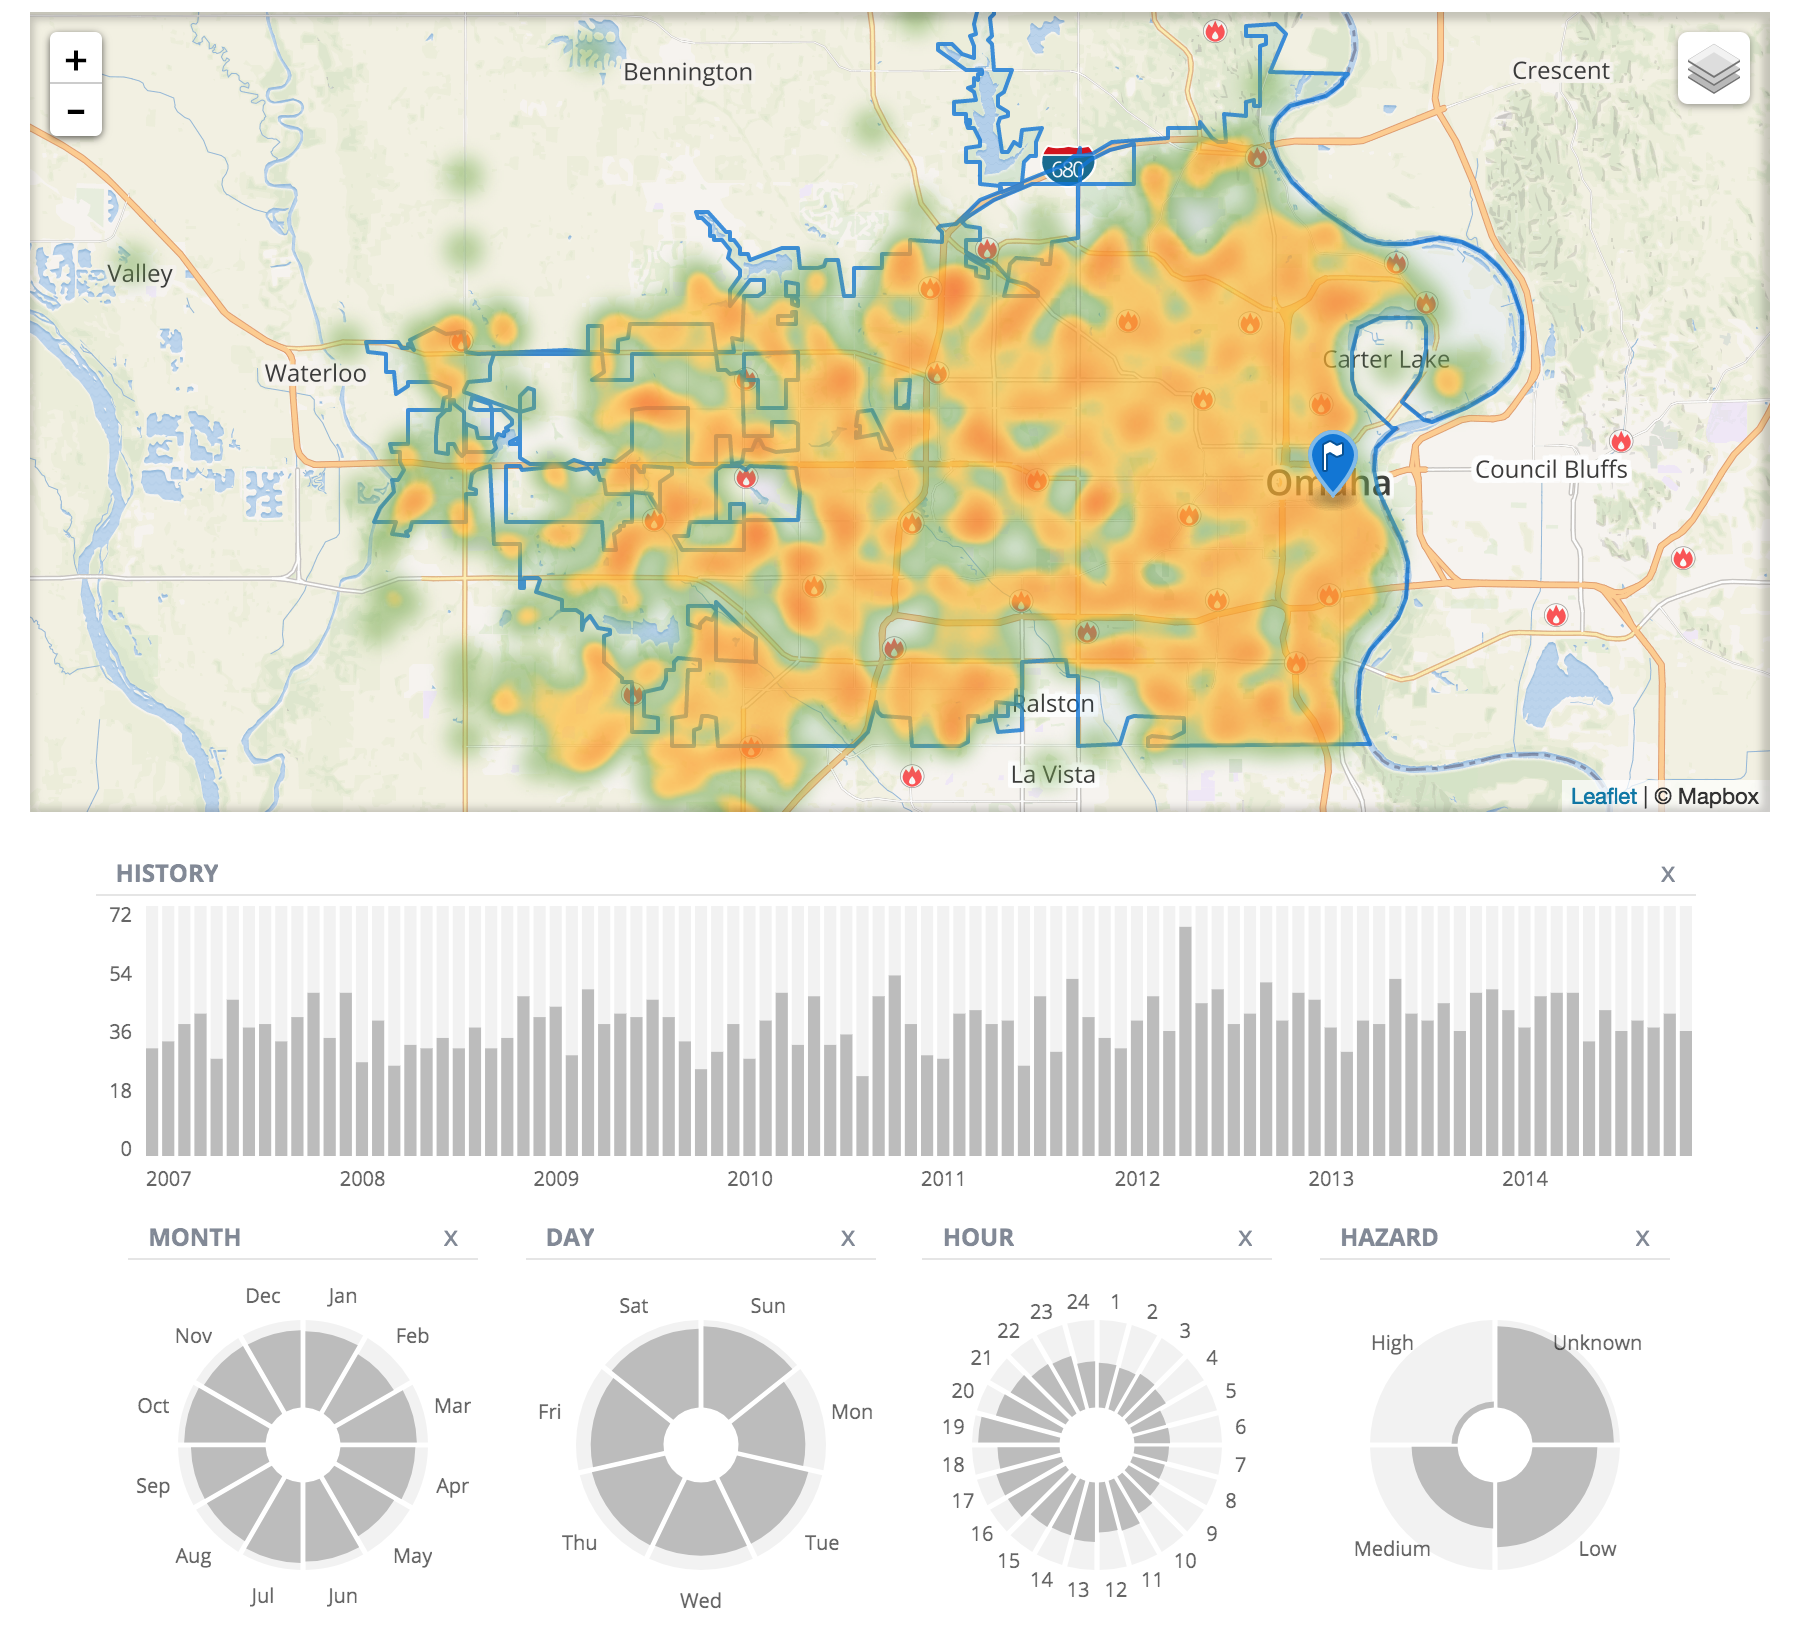
\includegraphics[width=.9\columnwidth]{Figures/interactive_fire_map}
\caption{Interactive geospatial map of fires that is sortable by time and parcel hazard level.}
\label{fig:interactive_fire_map}
\end{figure}

\section{Interactive Parcel Data}

\begin{figure}[ht!]
\centering
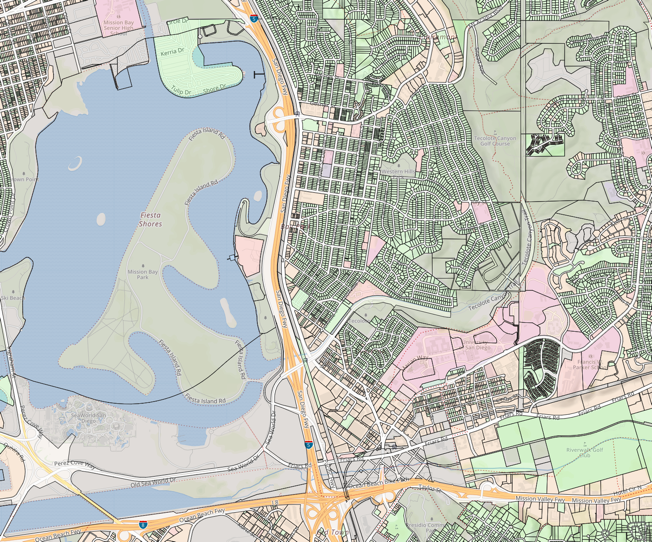
\includegraphics[width=.9\columnwidth]{Figures/parcel_data}
\caption{Interactive map showing hazard level of parcels as well as pacel specific information such as age, footprint, number of floors.}
\label{fig:parcel_data}
\end{figure}

\section{Predicted Fire Estimates}

\begin{figure}[ht!]
\centering
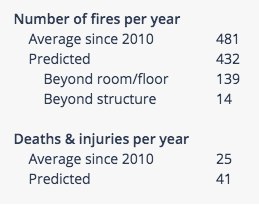
\includegraphics[width=.5\columnwidth]{Figures/fire_predictions}
\caption{Estimated prediction of number of fires, fire size, and number of causaulties.}
\label{fig:fire_predictions}
\end{figure}

\chapter{Updating Data}





\section{}



\end{document}
